
\section{Distribución de probabilidad discreta}

\subsection{Funciones de masa de probabilidad discretas (PMF y soporte)}

Supongamos que a cada punto del espacio muestral se le asigna un número.  Entonces hemos definido una \emph{función} en el espacio muestral.  Esta función es llamada \emph{variable aleatoria} (o \emph{variable estocástica}) o de manera más precisa \emph{función aleatoria}. 


Usualmente, las variables aleatorias se denotan por letras mayúsculas como $X$ o $Y$. En general, una variable aleatoria tiene algún significado físico, geométrico, económico, financiero, etc.



\begin{ejemplo}
	\label{exmp:2.6.1}
	Supongamos que una moneda se lanza dos veces de manera que el espacio muestral es $\set{HH,HT,TH,TT}.$  Digamos que $X$ representa el número de soles ($H$) que obtenemos.
\end{ejemplo}


\subsubsection{Funciones de probabilidad discretas}

Sea $X$ una variable aleatoria discreta.  Supongamos que los valores que puede tomar son $x_{1},...,x_{k},$ arreglados en algún orden dado.  Supongamos también que esos valores
tienen alguna probabilidad dada por
\begin{align}
	\label{eq:2.6.1}
	P(X=x_{k})=f(x_{k}).
\end{align}


{Función de probabilidad}
\begin{align}
	\label{2.2}
	P(X=x)=
	\begin{cases}
		f(x) & x=x_{k} \\
		0	& \text{en otro caso}
	\end{cases}
\end{align}



En general, $f(x)$ será una función de probabilidad si
\begin{align}
	\begin{cases}
		f(x)\geq 0 \\
		\sum_{x}f(x)=1.
	\end{cases}
\end{align}



\begin{ejemplo}
	\label{exmp:2.6.2}
	Encuentre la función de probabilidad correspondiente a la variable aleatoria $X$ del ejemplo \ref{exmp:2.6.1}.
\end{ejemplo}

\begin{solucion}
	El espacio muestral es $\{HH, HT, TH, TT\}$, cada uno con probabilidad $\frac{1}{4}$.
	
	$X$ = número de soles ($H$):
	\begin{itemize}
		\item $X = 0$ para $TT$: $P(X=0) = \frac{1}{4}$
		\item $X = 1$ para $HT, TH$: $P(X=1) = \frac{2}{4} = \frac{1}{2}$
		\item $X = 2$ para $HH$: $P(X=2) = \frac{1}{4}$
	\end{itemize}
	
	La función de probabilidad es:
	\begin{align}
		f(x) = \begin{cases}
			\frac{1}{4} & x = 0 \\
			\frac{1}{2} & x = 1 \\
			\frac{1}{4} & x = 2 \\
			0 & \text{en otro caso}
		\end{cases}
	\end{align}
\end{solucion}



\begin{ejemplo}
	\label{exmp:2.6.3}
	Suponga que un par de dados se lanzan. Sea $X$ la variable aleatoria dada por la suma de los puntos. Encuentre la distribución de probabilidad de $X.$
\end{ejemplo}

\begin{solucion}
	El espacio muestral tiene $6 \times 6 = 36$ resultados. La variable $X$ toma valores de 2 a 12.
	
	\begin{align}
		f(x) = P(X=x) = \frac{\text{número de formas de obtener } x}{36}
	\end{align}
	
	\begin{center}
	\begin{tabular}{c|ccccccccccc}
		$x$ & 2 & 3 & 4 & 5 & 6 & 7 & 8 & 9 & 10 & 11 & 12 \\
		\hline
		$f(x)$ & $\frac{1}{36}$ & $\frac{2}{36}$ & $\frac{3}{36}$ & $\frac{4}{36}$ & $\frac{5}{36}$ & $\frac{6}{36}$ & $\frac{5}{36}$ & $\frac{4}{36}$ & $\frac{3}{36}$ & $\frac{2}{36}$ & $\frac{1}{36}$
	\end{tabular}
	\end{center}
\end{solucion}



\begin{ejemplo}
	\label{exmp:2.6.4}
	Encuentre la distribución de probabilidad de niños y niñas en familias con 3 hijos, suponiendo la misma probabilidad para niños y niñas.
\end{ejemplo}

\begin{solucion}
	Sea $X$ = número de niños. Cada hijo es niño (N) o niña (M) con probabilidad $\frac{1}{2}$.
	
	El espacio muestral tiene $2^3 = 8$ resultados: $\{NNN, NNM, NMN, NMM, MNN, MNM, MMN, MMM\}$.
	
	$X$ puede tomar valores 0, 1, 2, 3:
	\begin{align}
		f(x) = \begin{cases}
			\frac{1}{8} & x = 0 \text{ (MMM)} \\
			\frac{3}{8} & x = 1 \text{ (NMM, MNM, MMN)} \\
			\frac{3}{8} & x = 2 \text{ (NNM, NMN, MNN)} \\
			\frac{1}{8} & x = 3 \text{ (NNN)}
		\end{cases}
	\end{align}
	
	Este es un ejemplo de distribución binomial con $N=3$ y $p=\frac{1}{2}$.
\end{solucion}



\subsection{Función de distribución acumulada para variables aleatorias discretas (CDF)}


La función de distribución de una variable discreta $X$ se obtiene de la función de probabilidad a través de la siguiente fórmula
\begin{align}
	\label{eq:2.6.2}
	F(x) = P(X\leq x) = \sum_{u \leq x} f(u).
\end{align}



Si $X$ toma sólo un número finito de valores $x_{1},...,x_{n}$ entonces la función de distribución está dada por
\begin{align}
	\label{eq:2.6.3}
	F(x)=
	\begin{cases}
		0 & -\infty < x < 0 \\
		f(x_{1}) & x_{1} \leq x < x_{2} \\
		f(x_{1})+f(x_{2}) & x_{2} \leq x < x_{3} \\
		\vdots & \vdots \\
		f(x_{1})+\cdots+f(x_{n}) & x_{n} \leq x < \infty
	\end{cases}
\end{align}



\begin{ejemplo}
	\label{exmp:2.6.5}
	Encuentre la función de distribución para la variable aleatoria $X$ del ejemplo \ref{exmp:2.6.2} y obtenga su gráfica.
\end{ejemplo}



\begin{figure}
	\centering
	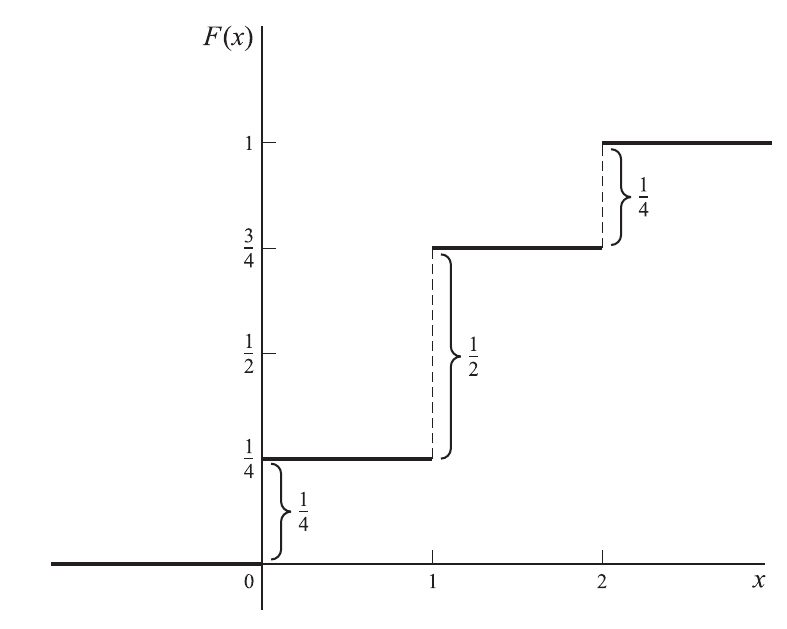
\includegraphics[height=7cm,keepaspectratio=true]{./pe/pands0201.png}
	% pands0201.png: 0x0 pixel, 300dpi, 0.00x0.00 cm, bb=
	\label{fig:2.6.1}
\end{figure}



\begin{observacion}
	\begin{itemize}
		\item Los saltos en la función de distribución están determinados por el valor de la función de probabilidad. 
		\item Este tipo de funciones se conoce como \emph{función escalonada}.  Debe observarse que son \emph{continuas por la derecha.}
		\item La función de distribución es \emph{monótonamente creciente.}
	\end{itemize}
	
\end{observacion}



La función de probabilidad se puede obtener a partir de la función de distribución con la siguiente fórmula
\begin{align}
	\label{eq:2.6.4}
	f(x)=F(x)-\lim_{u \to x^{-}}F(u).
\end{align}



\begin{ejemplo}
	\label{exmp:2.6.6}
	\begin{enumerate}
		\item Encuentre la función de distribución $F(x)$ para la variable aleatoria del problema resuelto \ref{exmp:2.6.3};
		\item grafique esta función de distribución.
	\end{enumerate}

\end{ejemplo}



\begin{figure}
	\centering
	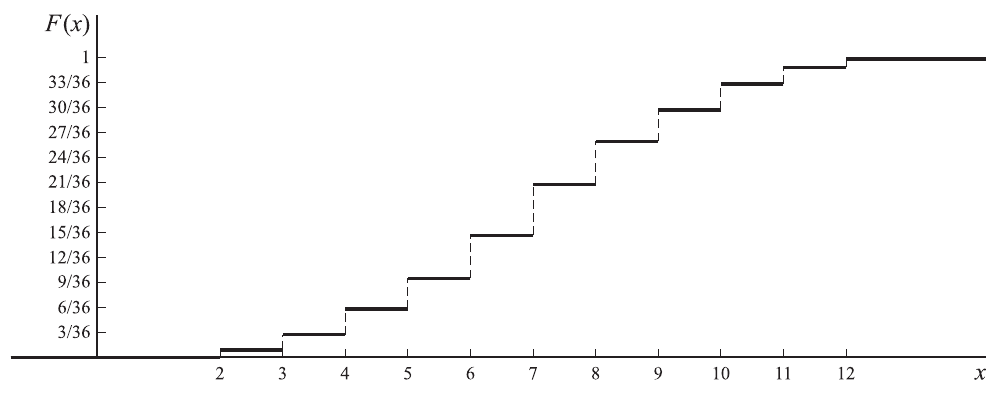
\includegraphics[width=10cm,keepaspectratio=true]{./pe/pands0206.png}
	% pands0206.png: 0x0 pixel, 300dpi, 0.00x0.00 cm, bb=
	\label{fig:2.6.2}
\end{figure}




\begin{ejemplo}
	\label{exmp:2.6.7}
	\begin{enumerate}
		\item Encuentre la función de distribución $F(x)$ para la variable aleatoria del problema resuelto \ref{exmp:2.6.4};
		\item grafique esta función de distribución.
	\end{enumerate}

\end{ejemplo}



\begin{figure}
	\centering
	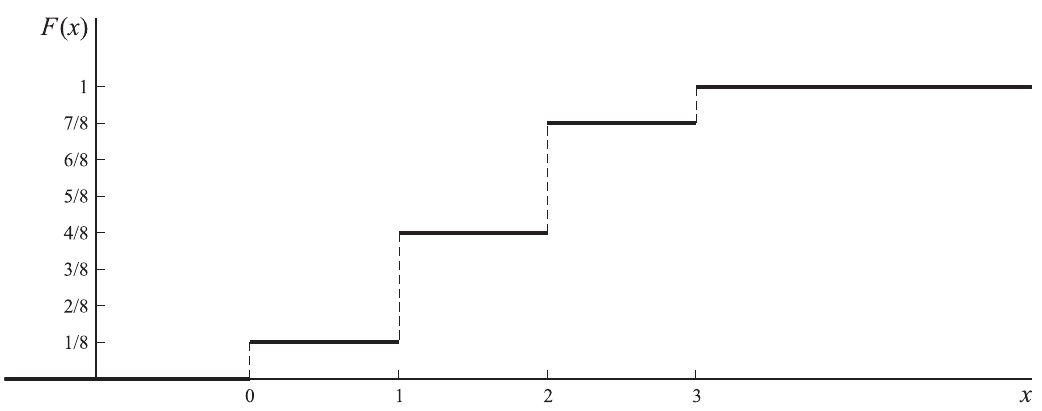
\includegraphics[width=10cm,keepaspectratio=true]{./pe/pands0207.png}
	% pands0206.png: 0x0 pixel, 300dpi, 0.00x0.00 cm, bb=
	\label{fig:2.6.3}
\end{figure}

\subsection{Esperanza matemática y varianza en variables aleatorias discretas}

\subsubsection{Valor esperado de una variable aleatoria discreta}
Para una variable aleatoria discreta $X$ con función de masa de probabilidad $f(x) = P(X=x)$ y soporte $S_X = \set{x_1, x_2, \dots, x_n, \dots}$, la \emph{esperanza matemática} o \emph{valor esperado} se define como el promedio ponderado de sus posibles valores:
\begin{align}
	\label{eq:esperanza_discreta}
	\mu = \mathbb{E}[X] = \sum_{x \in S_X} x f(x).
\end{align}
La esperanza matemática existe si y solo si la suma converge absolutamente ($\sum_{x \in S_X} |x| f(x) < \infty$). Físicamente, el valor esperado representa el centro de masa de la distribución de probabilidad en la recta numérica.

\subsubsection{Varianza y desviación estándar discretas}
La \emph{varianza} de una variable aleatoria discreta mide la dispersión cuadrática media respecto a la esperanza $\mu$:
\begin{align}
	\label{eq:varianza_discreta}
	\sigma^2 = \s^2 = \Var(X) = \mathbb{E}\left[(X - \mu)^2\right] = \sum_{x \in S_X} (x - \mu)^2 f(x).
\end{align}
Mediante linealidad del operador esperanza, la fórmula computacional abreviada para la varianza es:
\begin{align}
	\label{eq:varianza_formula_corta}
	\Var(X) = \mathbb{E}[X^2] - (\mathbb{E}[X])^2 = \sum_{x \in S_X} x^2 f(x) - \mu^2,
\end{align}
donde $\mathbb{E}[X^2]$ es el segundo momento bruto de la variable. La desviación estándar es la raíz cuadrada de la varianza: $\sigma = \sqrt{\Var(X)}$.

